\chapter{Results}\label{chapter:results}
Following the production of the BDT discriminator shapes for data and the simulated samples and their shape systematic uncertainties, a simultaneous fit of these shapes was performed and evaluated to determine the observed signal strength and measure the cross section.

\section{Statistical Methodology}\label{sec:statisticalModel}
The statistical methodology used for the search presented used the Higgs Analysis Combined Limit (\combine) tool~\cite{Combine} tool, a framework based on the RooStats package~\cite{Moneta:2010pm,Schott:2012zb}.

The \combine tool 
These statistical significances were determined using a binned Maximum Likelihood Fit (MLF)



 using Higgs Analysis Combined Limit (\combine) tool~\cite{Combine},

The \combine tool was used to determine the signal strength through a binned Maximum Likelihood Fit (MLF) and the significances using using an asymptotic approximation~\cite{AsymptoticFormulae}, using the Asimov dataset.

As it is assumed that the number of events in any given bin will be distributed according to Poisson statistics, the 


The likelihood function is the product of the Pois

Poisson = known constant rate and independently of the time since the last event

\begin{equation}
L = \prod\limits_{i=1}^{\N} _{i} \frac{•}{•} \;
\label{eq:poissonLikelihood}
\end{equation}

\begin{equation}
\mathcal{L} = - L = \sum\limits_{i=1}^{\N} _{i} \frac{\mu_{i}}{•} \;
\label{eq:minLogLikelihood}
\end{equation}

In the following section the signal and background yields are referred to as $s$ and $b$ respectively, where both represent event counts in the probability distribution function bins.
The uncertainties for the simulated 

All the systematic uncertainties were incorporated into the fit as nuisance parameters.
The normalisation uncertainties are incorporated into the fit as log-normal nuisance parameters

All the source of systematic uncertainty was incorporated into the fit as nuisance parameters, represented by $\theta$.
The shape uncertainties are incorporated into the fit by vertically morphing ~\cite{Baak:2014fta} the nominal shape template up and down 
Normalisation uncertainties are 

All sources of uncertainties have been assumed to be either 100\% correlated or uncorrelated.
Uncertainties which are partially correlated have been broken down into subcomponents so that they can be declared either 100\% correlated or uncorrelated.
This allows all constraints to be included in the likelihood functions in a clean factorised form. 

Gross:2007zz - LHC stats for pedestraians

\subsection{Confidence Levels Method}\label{subsec:CLs}
The modified classical frequentist method known as the CL$_{s}$ was used to set limits on the strength of the signal process.
A test statistic, $q_{\mu}$, is defined to discriminate between 
confidence levels are determined on modified classical frequentist methods 


The test statistic most commonly used by the ATLAS and CMS collaborations is defined in equation~\ref{eq:testStatistic} as:

\begin{equation}
\q_{\mu} =  -2 \ln \frac{ \mathcal{L}(data | \mu s , \hat{\theta_{\mu}}}{ \mathcal{L}(data | \hat{\mu} s \hat{\theta_{\mu}},  } \;
\label{eq:testStatistic}
\end{equation}

where the
$\hat{\mu}$ 
cannot take negative values as physics defines the signal rate as positive.
In addition, 


The \emph{Asymptotic} CL$_{s}$ method is typically used 
This method uses one representive dataset, known as the \emph{Asimov dataset}, in lieu of an ensemble of toy MC samples.
The Asimov dataset is constructed such that ...
A full description of this methodology is given in~\cite{Cowan:2010js}.

\subsection{Data-driven background normalisation}\label{subsec:combineNormalisation}
floating in the fit



\section{Impact of the Systematic Uncertainties}\label{sec:uncertainitiesImpact}
The effect of each of the sources of systematic uncertainty considered in terms of the pull ($\frac{ \hat{\theta} - \theta_{0} }{\Delta \theta}$) and the postfit impact of varying the sources of uncertainty by $\pm 1 \sigma$ are shown in figure~\ref{fig:systematicsPull}.

\editComment{Remark on the lumi, jer are the largest uncerts and how the rest of the experimental uncerts are considerably smaller}

\begin{figure}[htbp]
\begin{center}
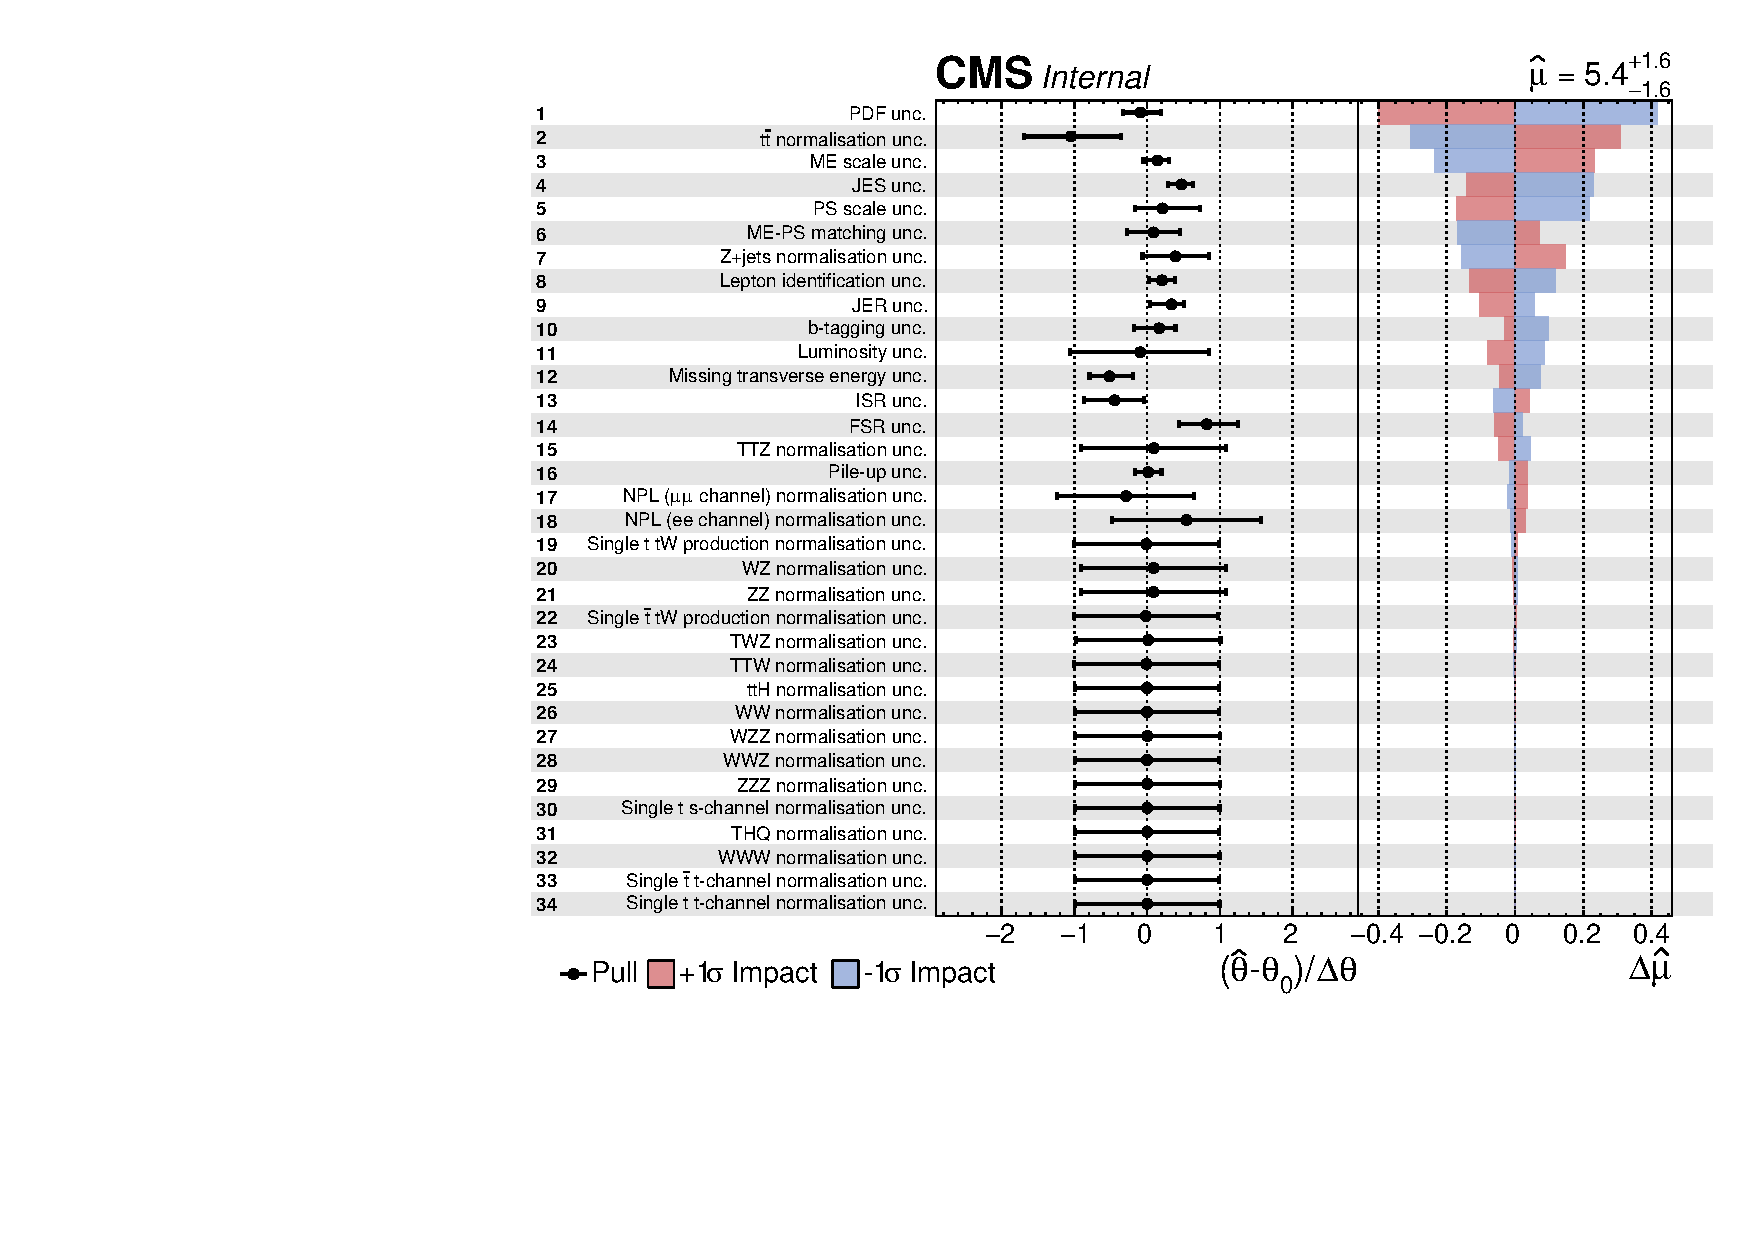
\includegraphics[width=0.97\textwidth]{figs/results/systematicsImpact.pdf}
\caption{The impact of each of the systematic uncertainties considered on the measurement made.}
\label{fig:systematicsPull}
\end{center}
\end{figure}

\section{Cross section extraction}
The cross section is 

By performing a simultaneous fit of the BDT discriminant distribution for the background-enriched sample and the BDT discriminant in the signal sample, any events in excess of the background-only hypothesis will be determined.

This excess can then be compared to the SM expectation for tZq production in order to calculate the observed signal strength and measure the cross section.

A measured signal strength of 0.0 would correspond to an observation of the background-only hypothesis alone, whilst 1.0 is the SM expectation for tZq sproduction.

\section{Statistical Analysis Results}
\editComment{UPDATE BEFORE SUBMISSION}
For the combination of both of the final states, at the 95\% CL, the cross section for tZq production was measured to be $X^{+Y}_{-Z}$, which is within the uncertainties of the SM prediction.
This result corresponds to an observed significance of $X_{-Z}^{+Y} \sigma$ against an expected significance of $X_{-Z}^{+Y} \sigma$.

The observed signal strengths, measured cross sections, and corresponding significances for the individual channels and their combination are shown in full in table~\ref{tab:shapetxs}.

These results are [IN AGREEMENT / NOT IN AGREEMENT] with the SM cross section of  $X^{+Y}_{-Z}$.

\begin{table}[!h]
   \centering
   \caption{The observed signal strengths and corresponding cross sections for
   the individual channels and the channels combined at the 95\% CL.}
   \begin{tabular}{cccc}
       \hline
       Channel & $ee$ & $\mu\mu$ & \textbf{Combination} \\
        \hline
       Signal strength & $X_{-Z}^{+Y}$ & $X_{-Z}^{+Y}$ & $X_{-Z}^{+Y}$ \\
       Cross section (fb) & $X_{-Z}^{+Y}$ & $X_{-Z}^{+Y}$ & $X_{-Z}^{+Y}$ \\
       Significance (expected) ($\sigma$) & $X_{-Z}^{+Y}$ & $X_{-Z}^{+Y}$ & $X_{-Z}^{+Y}$ \\
       Significance (observed) ($\sigma$) & $X_{-Z}^{+Y}$ & $X_{-Z}^{+Y}$ & $X_{-Z}^{+Y}$ \\
    \end{tabular}
   \label{tab:shapetxs}
\end{table}

At the time of writing this thesis, discussions were being undertaken on how best to take this search forward.
The two options under consideration were resenting it as a standalone search or a combination with the trilepton search following the inclusion of data collected by the CMS detector during 2017.
As such, while the result presented here is not a final result, an updated result is intended presented in a future CMS publication in the near future.

\section{Discussion of other searches for tZq at the Large Hadron Collider}
The search for the dilepton final state of a singly produced top in association with a Z boson presented in this thesis is the first one that has been undertaken at the LHC.
As such while these results cannot be compared against any previous or competing results, searches for tZq have been made for the trilepton final state at $\sqrt{s} = 8 \TeV and 13 \Tev$.

Following the trilepton tZq search at $\sqrt{s} = 8 \TeV$ by the CMS collaboration which reported a significance of 2.9 standard deviations ~\cite{Sirunyan:2017kkr}, at $\sqrt{s} = 13 \TeV$ both the ATLAS and CMS collaborations  have reported significances in excess of 3.0 standard deviations, 4.2 and 3.7 respectively~\cite{Aaboud:2017ylb,Sirunyan:2017nbr}.

Despite the dilepton final state having a larger production cross section than the fully leptonic final state, given that the topology of the dilepton final state results in an increased difficulty in rejecting background processes, 


Given that the search for the dilepton final state is currently statistically limited, it is anticipated that including data collected by the CMS experiment during 2017 could allow for a significance close to or in excess of 3.0 standard deviations to be observed.
Even if additional statistics isn't sufficient for an observation to be made of the dilepton final state, when combined with the trilepton final state result, it is expected that the discovery of tZq should be possible.